\documentclass[11pt]{article}

\usepackage[margin=2.5cm]{geometry}
\usepackage{graphicx}
\usepackage{booktabs}
\usepackage{amsmath}
\usepackage{caption}
\usepackage{float}
\usepackage[hidelinks]{hyperref}

\graphicspath{{figures/}}
\captionsetup{font=small, labelfont=bf, width=0.92\textwidth}

% Long unbreakable code tokens: allow a little inter-word stretch instead of
% letting lines run into the margin.
\emergencystretch=1.5em

\newcommand{\code}[1]{\texttt{#1}}

\title{Market Regime Detection and the Robustness of Simple\\
Allocation Strategies\\[0.6em]
\large A reproducible walk-forward study (RegimeLab, v3)}
\author{Mohamed Ryadi}
\date{June 2026}

\begin{document}

\maketitle

\begin{abstract}
\noindent
We study whether market regime detection improves the \emph{robustness} ---
rather than the headline performance --- of simple allocation strategies,
out-of-sample and net of transaction costs. Using a walk-forward framework on
the S\&P~500 ETF (SPY, 2005--2026) with proportional costs and a T-bill cash
leg, we compare buy-and-hold and trend-following baselines against variants
gated by a transparent volatility filter and by 2- and 3-state Gaussian hidden
Markov models (HMMs) restricted to \emph{filtered} state probabilities. Regime
gating raises the excess-return Sharpe ratio from 0.55 to about 0.70 and cuts
the maximum drawdown from $-55\%$ to between $-33\%$ and $-17\%$. However,
paired block-bootstrap intervals show that \emph{no Sharpe difference is
statistically distinguishable from zero at the 95\% level}; the Sharpe edge
concentrates in crisis eras, while the drawdown reduction is consistent across
all eras. On a diversified SPY/TLT/GLD portfolio, no gate beats equal-weight
buy-and-hold. The HMM never outperforms the volatility heuristic, and its
filtered-state flicker triples turnover; a simple no-trade band repairs this,
taking the HMM family from clearly worse than the diversified benchmark
(Sharpe 0.64) to nearly matching it (0.79) with half the maximum drawdown. We
conclude that regime detection is best understood as crash insurance, that
model complexity must earn its costs and here does not, and that all findings
are stable across bootstrap block lengths and walk-forward schedules.
\end{abstract}

\section{Introduction and research question}

Regime-switching ideas are pervasive in quantitative asset allocation:
markets appear to alternate between calm and turbulent states, and
conditioning exposure on the current state should, in principle, improve
risk-adjusted outcomes. Published evidence, however, is often contaminated by
look-ahead bias (smoothed rather than filtered state estimates), in-sample
parameter selection, and ignored transaction costs.

RegimeLab is a research platform built to ask the question under deliberately
conservative conditions. Three questions structure the study:

\begin{enumerate}
  \item Does regime detection improve the \emph{robustness} of simple
        strategies --- out-of-sample, net of costs, with cash properly
        compensated --- rather than their in-sample performance?
  \item Does a statistical regime model (a Gaussian HMM) earn its complexity
        relative to a transparent volatility heuristic?
  \item Do the answers survive diversification across asset classes, and can
        the cost side of regime trading be repaired mechanically?
\end{enumerate}

The contribution is methodological as much as empirical: every defense
against look-ahead bias is structural (encoded once, in one place, and
tested), every experiment is reproducible from a configuration file and a
seed, and every methodological decision is recorded in a public decision log.

\section{Data}

\textbf{Prices.} Daily adjusted closes from Yahoo Finance, cached immutably
with JSON sidecars recording source and download date. The single-asset
universe is SPY from January 2000; the multi-asset universe adds long-duration
Treasuries (TLT) and gold (GLD) from December 2004 (GLD inception).

\textbf{Cash rate.} The 13-week T-bill yield index (\code{\textasciicircum
IRX}), converted from an annualized percentage to a daily simple return as
$y/100/252$ (a documented approximation), forward-filled over bond-market
holidays on a continuous business-day calendar, and \emph{lagged one day}: the
rate known at the close of $t$ accrues over $t{+}1$. Over the out-of-sample
window the cash leg averaged about $1.7\%$ per year.

\textbf{Returns.} Simple returns for portfolio aggregation; log returns for
statistical modeling.

\section{Methodology}

\subsection{Backtest protocol}

Let $w_t$ denote the vector of target portfolio weights decided at the close
of day $t$ (long-only, $\sum_i w_{i,t} \le 1$). The engine applies a one-day
execution lag --- strategies never lag their own signals, so the lag exists in
exactly one tested place:
\begin{equation}
  h_t = w_{t-1}, \qquad
  \tau_t = \sum_i \lvert h_{i,t} - h_{i,t-1} \rvert ,
\end{equation}
where $h_t$ are the weights actually held during $t$ and $\tau_t$ is the
turnover. The net portfolio return with proportional costs $c$ (in fractions
per unit turnover) and cash rate $r^f_t$ is
\begin{equation}
  r^p_t \;=\; \sum_i h_{i,t}\, r_{i,t}
  \;+\; \max\!\Bigl(0,\, 1 - \sum_i h_{i,t}\Bigr)\, r^f_t
  \;-\; c\,\tau_t ,
\end{equation}
with the floor ensuring leveraged weights are never credited the cash rate.
Costs use $c = 5$ basis points as the headline level and are swept over
$\{0, 5, 20\}$ bps in every experiment. Sharpe and Sortino ratios are computed
on returns in excess of $r^f_t$.

\subsection{Regime models}

All models implement one interface (fit on training prices; emit a causal
regime label per date) and are fitted \emph{per asset}.

\textbf{Volatility threshold (heuristic).} A date is labeled turbulent when
trailing 20-day realized volatility exceeds the 80\% quantile of the training
sample's volatility distribution; the quantile threshold is the only fitted
state. Both parameters are swept in robustness checks.

\textbf{Gaussian HMM.} A $K$-state HMM with Gaussian emissions
$r_t \mid s_t = k \sim \mathcal{N}(\mu_k, \sigma_k^2)$ on log returns,
estimated by EM with several seeded restarts (best in-sample likelihood kept;
convergence metadata recorded). Because EM state labels are arbitrary and
change across refits, states are relabeled by ascending variance, so state $0$
is always the calmest. Crucially, prediction uses only the \emph{filtered}
distribution, computed by the forward recursion
\begin{equation}
  \alpha_t(k) \;\propto\; \varphi\!\left(r_t;\, \mu_k, \sigma_k^2\right)
  \sum_{j=1}^{K} \alpha_{t-1}(j)\, A_{jk},
  \qquad
  P\!\left(s_t = k \mid r_{1:t}\right) = \alpha_t(k),
\end{equation}
implemented in log space. Library routines based on the Viterbi path or on
smoothed (forward--backward) probabilities condition on the full sample ---
i.e.\ on future data --- and are used for diagnostics only. Truncation tests
($\text{predict}(x_{1:t}) = \text{predict}(x)_{1:t}$ for all $t$) enforce
causality for every model.

\subsection{Strategies}

With $E(k) \in [0,1]$ a fixed a-priori exposure map (flat in the
highest-variance state, fully invested otherwise):
\begin{align}
  \text{hard gate:} \quad & w_t = b_t \cdot E\!\left(\hat{s}_t\right),
    \qquad \hat{s}_t = \arg\max_k P(s_t = k \mid r_{1:t}) \\
  \text{probability scaling:} \quad & w_t = b_t \cdot e_t,
    \qquad e_t = \sum_k E(k)\, P(s_t = k \mid r_{1:t}) \\
  \text{no-trade band:} \quad & w_t =
    \begin{cases}
      w_{t-1} & \text{if } \lvert b_t e_t - w_{t-1} \rvert \le \delta \\
      b_t\, e_t & \text{otherwise,}
    \end{cases}
\end{align}
where $b_t$ is the base strategy's weight (buy-and-hold or a 200-day
moving-average trend rule). The band recursion is forward-only and passes the
same truncation tests. The band level $\delta$ is \emph{reported as a sweep}
over $\{0.05, 0.10, 0.20\}$, never selected in-sample.

\subsection{Walk-forward validation}

Models are refitted on an expanding window: an initial training sample of
1{,}260 trading days ($\approx$ 5 years), refit every 252 days. Only
out-of-sample labels and probabilities --- stitched across refits --- ever
reach a strategy. This yields 22 refits on SPY (out-of-sample 2005-01-07 to
2026-06-09, 5{,}388 days) and 17 refits on the multi-asset universe
(2009-12-02 to 2026-06-09, 4{,}154 days). The out-of-sample window and cost
levels are identical for gated and ungated strategies, so differences are
attributable to the regime signal alone.

\subsection{Statistical inference}

A point difference between two Sharpe ratios is not a finding. We use a
\emph{paired circular block bootstrap}: indices are resampled in contiguous
21-day blocks (wrapping at the boundary), the same blocks are applied to both
return series (preserving cross-correlation), and 95\% percentile intervals
are formed over 2{,}000 draws. We also report
$P(\le 0)$, the fraction of bootstrap draws in which the Sharpe difference is
non-positive --- a descriptive bootstrap quantity, not a formal $p$-value.
Block length is itself swept over $\{5, 21, 63\}$ days as a nuisance check.

\section{Implementation}

The repository separates an installable, unit-tested library
(\code{src/regimelab/}: data, features, regimes, strategies, backtest engine,
validation, inference, plotting) from configuration-driven experiments
(\code{experiments/} + \code{configs/}); notebooks only load experiment
outputs and call shared plotting helpers. The test suite (102 tests) includes
dedicated look-ahead defenses: a clairvoyant-signal canary for the engine lag,
truncation causality tests for every feature and regime model, and
train-precedes-test assertions for the walk-forward splits. A regression guard
verified that the v3 additions (cash leg, bands) reproduce earlier results
exactly when disabled. All methodological decisions and their rationale are
recorded in \code{reports/decisions.md}.

\section{Results: single asset (SPY)}

Table~\ref{tab:spy} reports the out-of-sample headline results at 5~bps.
Figures~\ref{fig:spywealth} and \ref{fig:spydd} show the corresponding wealth
and drawdown paths.

\begin{table}[H]
\centering
\caption{SPY, out-of-sample 2005--2026, net of 5 bps, cash leg active. Sharpe
and Sortino are on excess returns; turnover is one-way, annualized.
\code{hmm2p\_bXX} denotes probability scaling with a no-trade band
$\delta = 0.XX$.}
\label{tab:spy}
\small
\begin{tabular}{lrrrrrr}
\toprule
Strategy & Ann.\ ret. & Ann.\ vol. & Sharpe & Sortino & Max DD & Turnover \\
\midrule
buy\_and\_hold   & 10.9\% & 19.0\% & 0.55 & 0.78 & $-55.2\%$ & 0.05$\times$ \\
trend\_200d      &  8.3\% & 11.6\% & 0.60 & 0.81 & $-20.9\%$ & 6.3$\times$ \\
vol20q80\_bh     & 10.3\% & 12.8\% & 0.70 & 0.95 & $-33.2\%$ & 3.4$\times$ \\
vol20q80\_trend  &  8.5\% & 11.1\% & 0.64 & 0.87 & $-20.9\%$ & 5.9$\times$ \\
hmm2\_bh         &  9.3\% & 11.4\% & 0.69 & 0.95 & $-21.4\%$ & 9.4$\times$ \\
hmm2\_trend      &  8.2\% & 10.3\% & 0.65 & 0.89 & $-17.2\%$ & 7.9$\times$ \\
hmm2p\_bh        &  8.8\% & 10.8\% & 0.67 & 0.93 & $-22.0\%$ & 11.2$\times$ \\
hmm2p\_b05\_bh   &  8.8\% & 10.7\% & 0.68 & 0.93 & $-22.0\%$ & 10.0$\times$ \\
hmm2p\_b10\_bh   &  8.6\% & 10.5\% & 0.68 & 0.93 & $-21.0\%$ & 8.8$\times$ \\
hmm2p\_b20\_bh   &  8.8\% & 10.1\% & 0.71 & 0.99 & $-16.8\%$ & 6.7$\times$ \\
hmm3\_bh         & 10.1\% & 17.1\% & 0.55 & 0.76 & $-51.8\%$ & 4.1$\times$ \\
\bottomrule
\end{tabular}
\end{table}

\begin{figure}[H]
\centering
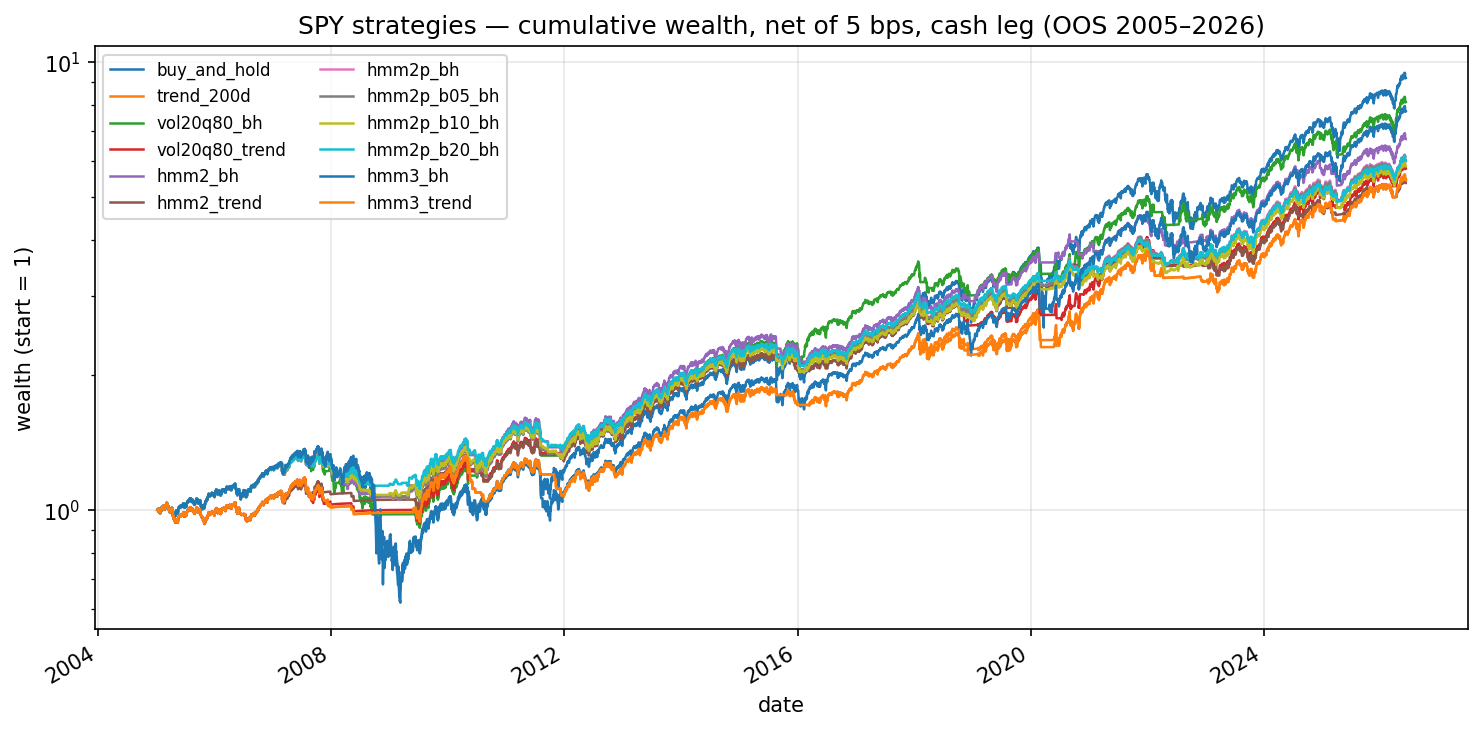
\includegraphics[width=\textwidth]{spy_wealth.png}
\caption{Cumulative wealth, net of 5 bps with the cash leg, out-of-sample
2005--2026 (log scale). Gated variants track buy-and-hold in calm markets and
step aside in turbulence: comparable terminal wealth with visibly shallower
paths through 2008--09, 2020, and 2022. The 3-state HMM gate
(\code{hmm3\_bh}) barely deviates from buy-and-hold because its extreme state
fires on only $2.5\%$ of days.}
\label{fig:spywealth}
\end{figure}

\begin{figure}[H]
\centering
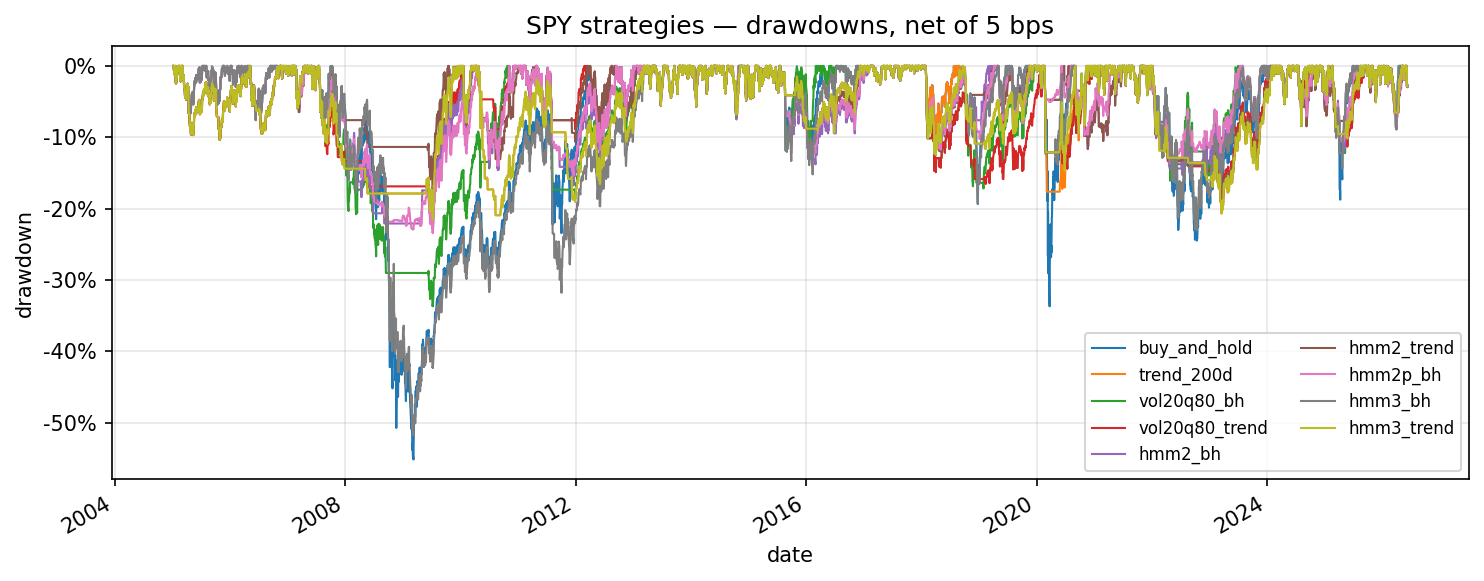
\includegraphics[width=\textwidth]{spy_drawdowns.png}
\caption{Drawdowns net of 5 bps. The headline effect of regime gating is
visible here rather than in terminal wealth: maximum drawdown improves from
$-55\%$ (buy-and-hold) to $-33\%$ (volatility gate) and $-17$ to $-22\%$ (HMM
variants).}
\label{fig:spydd}
\end{figure}

\subsection{What the HMM detects}

Figure~\ref{fig:regimes} overlays the out-of-sample turbulent labels
($21.0\%$ of days; the volatility filter flags $14.8\%$) on the SPY price,
with the filtered turbulence probability below. Labels concentrate on
2008--09, 2011, 2015--16, 2018, March 2020, and 2022. Near regime boundaries
the filtered probability oscillates around $0.5$; each oscillation is a round
trip for a hard-gated strategy. This \emph{filtered-state flicker} is the
mechanism behind the HMM's $9.4\times$ annual turnover and is the target of
the no-trade band.

\begin{figure}[H]
\centering
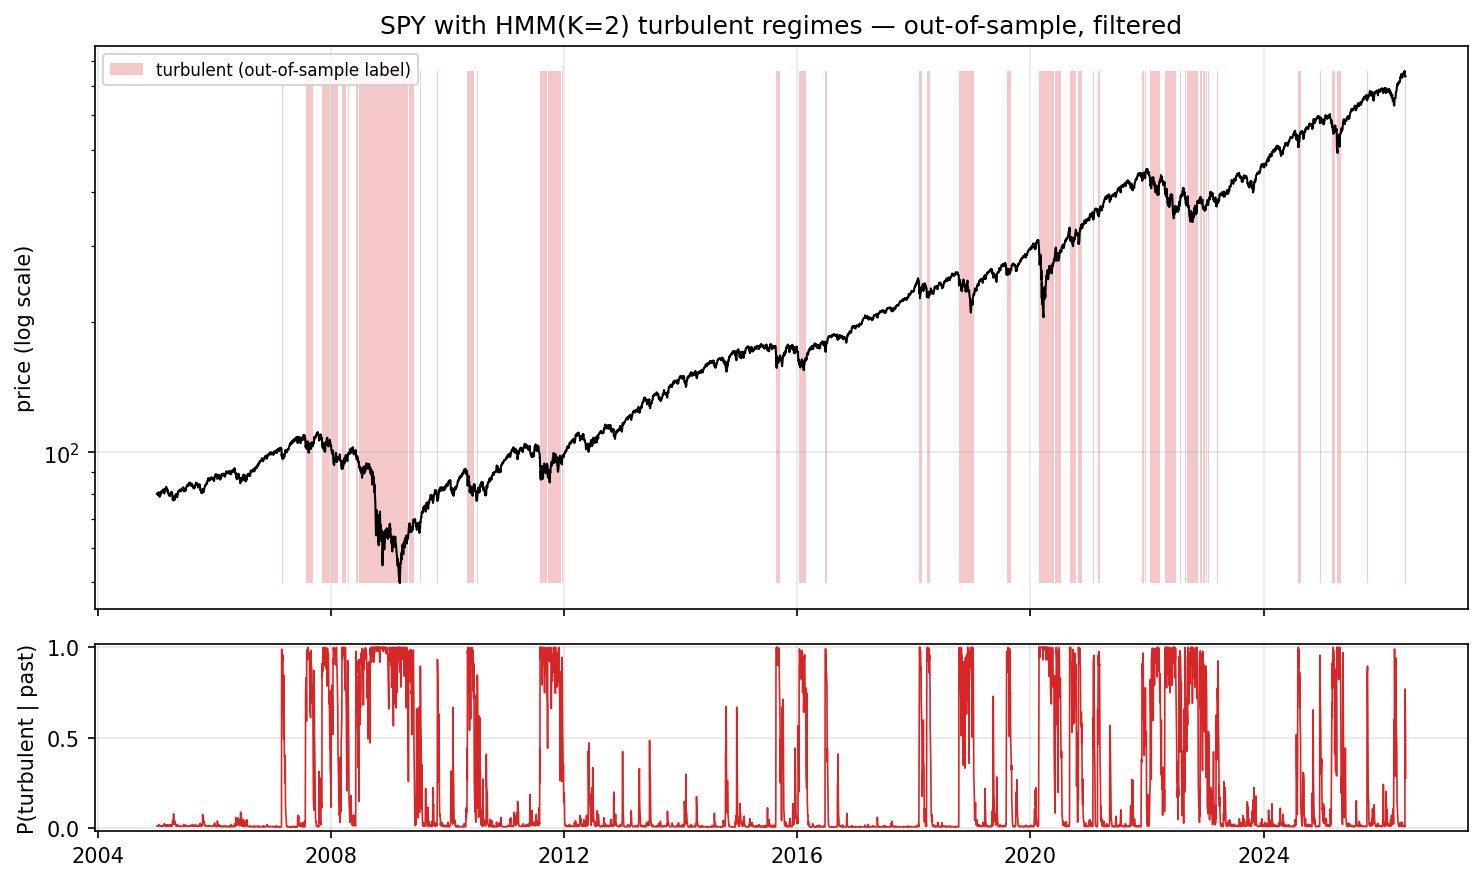
\includegraphics[width=\textwidth]{spy_hmm2_regimes.png}
\caption{SPY (log scale) with out-of-sample HMM($K{=}2$) turbulent regimes
shaded (top) and the filtered probability of the turbulent state (bottom).
Estimates at date $t$ use information up to $t$ only. The probability panel
shows the boundary flicker that drives turnover in hard-gated strategies.}
\label{fig:regimes}
\end{figure}

\subsection{Banding the flicker}

The band sweep cuts turnover monotonically ($11.2\times \to 10.0\times \to
8.8\times \to 6.7\times$) at no Sharpe cost; the widest band has the HMM
family's best Sharpe (0.71) and best maximum drawdown ($-16.8\%$)
(Figure~\ref{fig:spyfrontier}). We read this as a sweep result, not a tuned
point: the scaled strategy's Sharpe is flat in $\delta$ while its trading
costs are not, so banding is weakly dominant.

\begin{figure}[H]
\centering
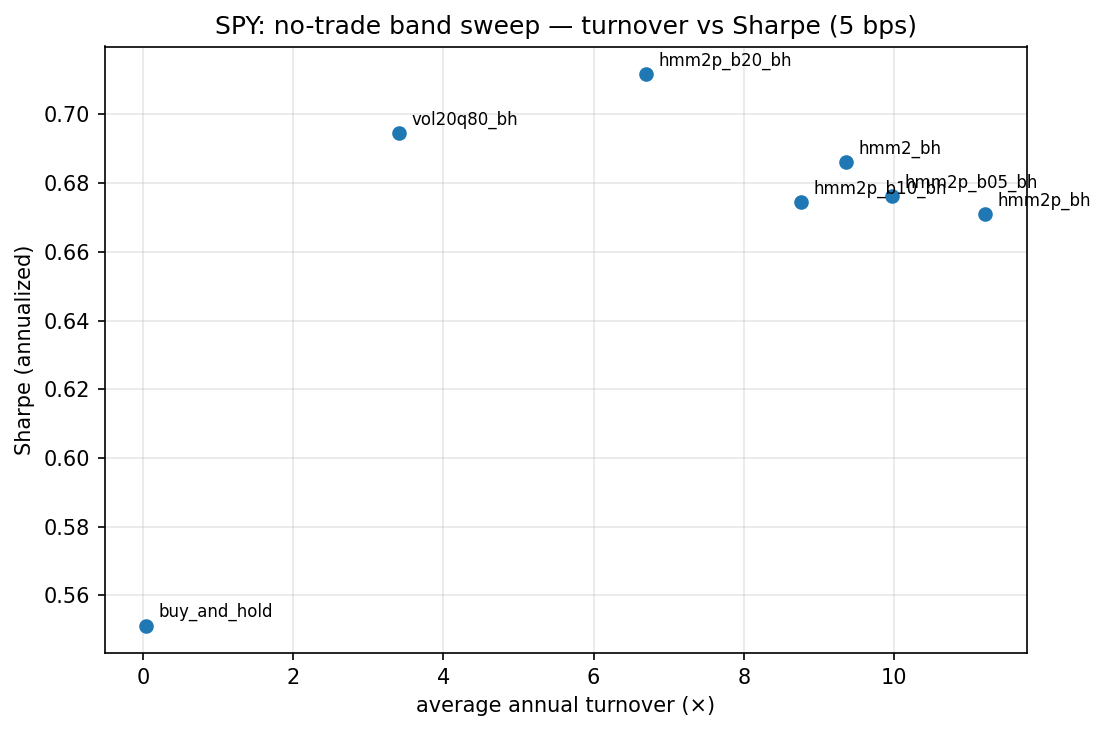
\includegraphics[width=0.8\textwidth]{spy_frontier.png}
\caption{Turnover versus Sharpe (SPY, 5 bps). Moving from the unbanded
probability-scaled strategy (\code{hmm2p\_bh}, right) through increasing band
levels traces an up-and-left path: less trading, equal or better
risk-adjusted performance.}
\label{fig:spyfrontier}
\end{figure}

\subsection{Is any of it statistically significant?}

\begin{table}[H]
\centering
\caption{Paired circular block bootstrap (21-day blocks, 2{,}000 draws) on
excess-return Sharpe differences, SPY at 5 bps. $P(\le 0)$ is the bootstrap
fraction of non-positive differences (descriptive).}
\label{tab:spyboot}
\small
\begin{tabular}{lrrr}
\toprule
Comparison & $\Delta$Sharpe & 95\% CI & $P(\le 0)$ \\
\midrule
vol20q80\_bh vs.\ buy\_and\_hold  & $+0.14$ & $[-0.15,\, +0.46]$ & 0.19 \\
hmm2\_bh vs.\ buy\_and\_hold      & $+0.14$ & $[-0.18,\, +0.48]$ & 0.24 \\
hmm2p\_b20\_bh vs.\ buy\_and\_hold& $+0.16$ & $[-0.15,\, +0.49]$ & 0.18 \\
hmm3\_bh vs.\ buy\_and\_hold      & $-0.01$ & $[-0.15,\, +0.16]$ & 0.57 \\
vol20q80\_bh vs.\ hmm2\_bh        & $+0.01$ & $[-0.21,\, +0.22]$ & 0.48 \\
hmm2\_bh vs.\ hmm2p\_bh           & $+0.02$ & $[-0.08,\, +0.11]$ & 0.38 \\
\bottomrule
\end{tabular}
\end{table}

Every 95\% interval includes zero (Table~\ref{tab:spyboot},
Figure~\ref{fig:spyboot}): twenty-one years of daily data cannot certify a
Sharpe improvement of $\approx 0.15$. The volatility heuristic and the 2-state
HMM are statistically indistinguishable from each other.

\begin{figure}[H]
\centering
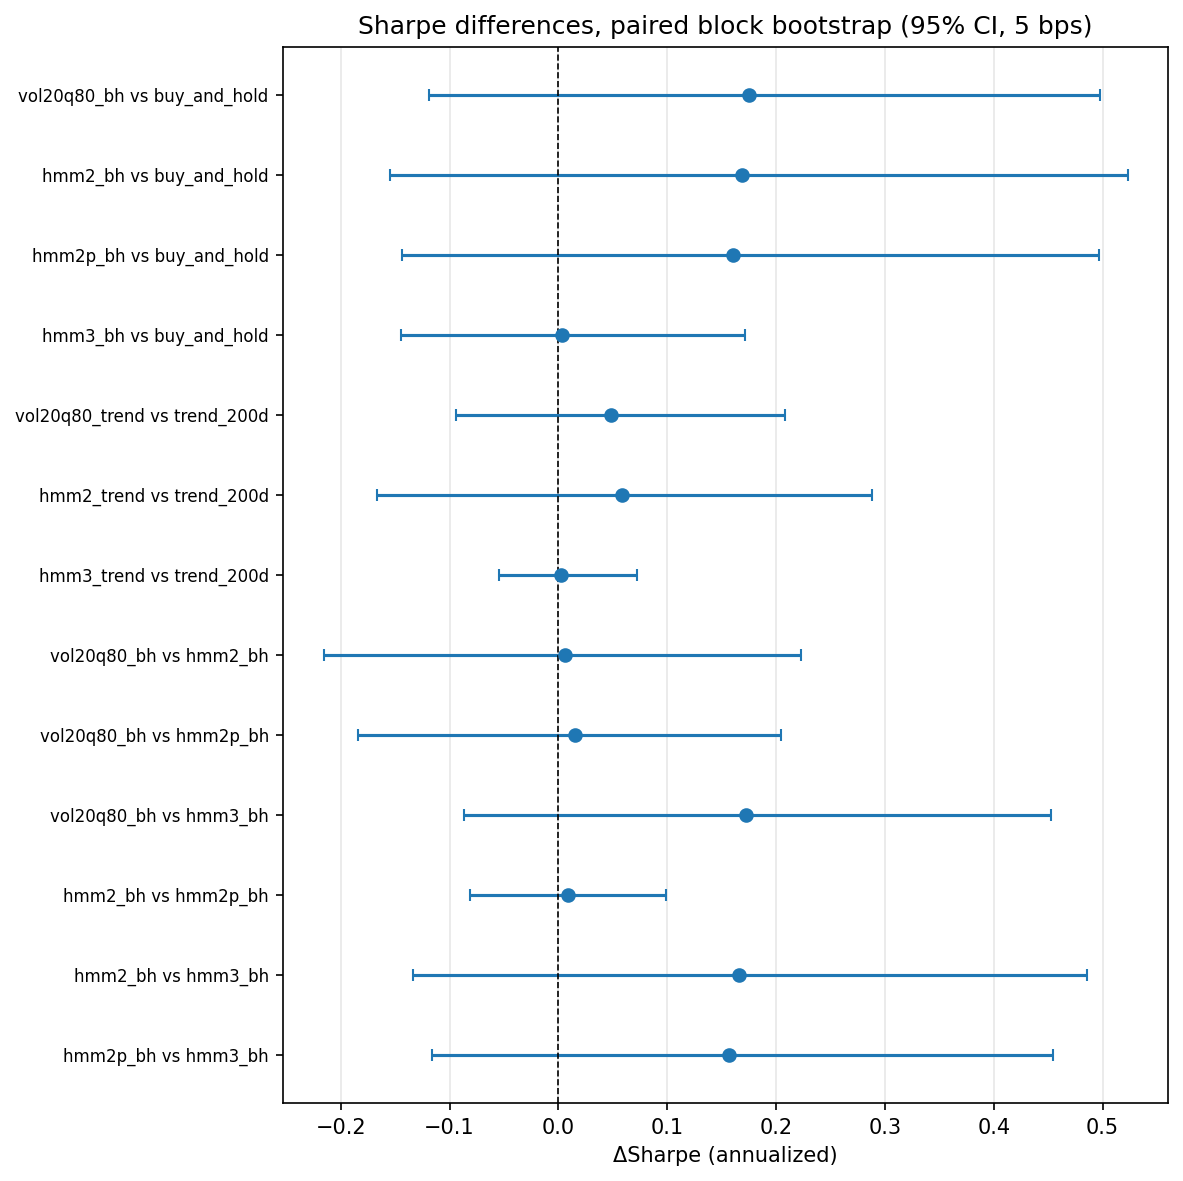
\includegraphics[width=0.85\textwidth]{spy_bootstrap.png}
\caption{Sharpe differences with 95\% paired-bootstrap intervals (SPY, 5 bps,
excess returns). All intervals straddle zero.}
\label{fig:spyboot}
\end{figure}

\subsection{Sub-periods, parameters, and nuisance choices}

\begin{figure}[H]
\centering
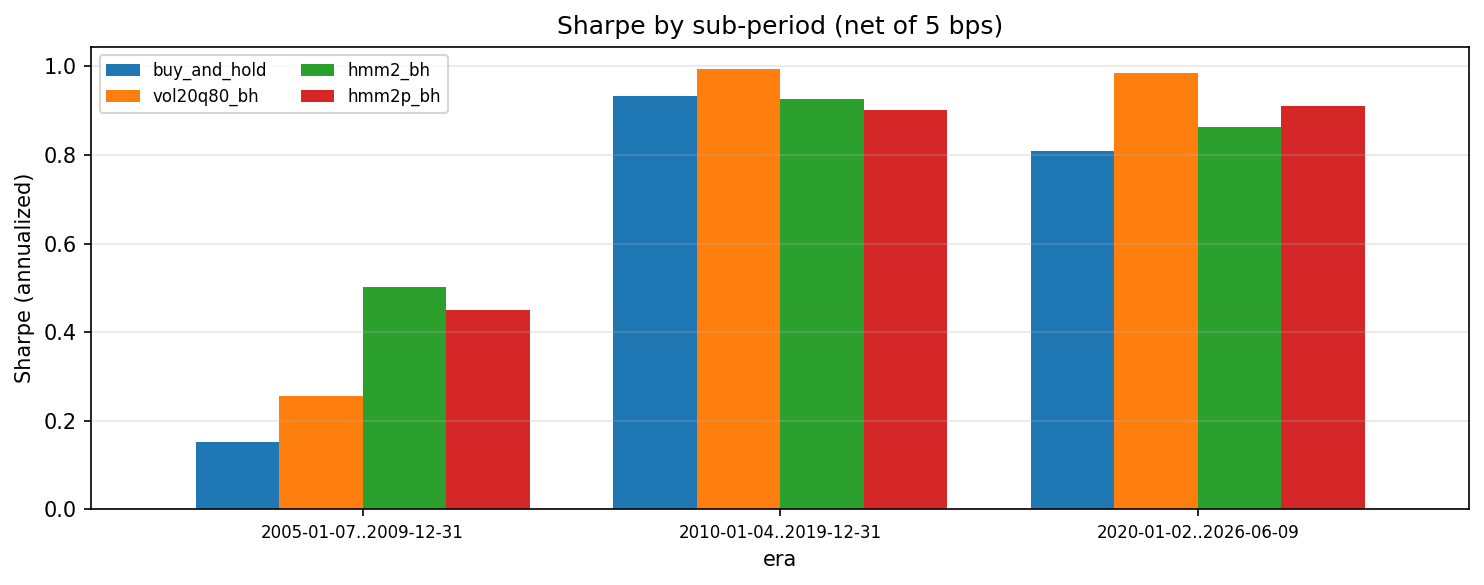
\includegraphics[width=0.95\textwidth]{spy_subperiods.png}
\caption{Excess Sharpe by sub-period. The Sharpe edge of gating lives in the
2005--09 crisis era (e.g.\ buy-and-hold 0.04 vs.\ \code{hmm2\_bh} 0.30) and
partially in 2020+; in the calm 2010s gating neither helped nor hurt. The
drawdown reduction (not shown) appears in every era.}
\label{fig:subperiods}
\end{figure}

\begin{figure}[H]
\centering
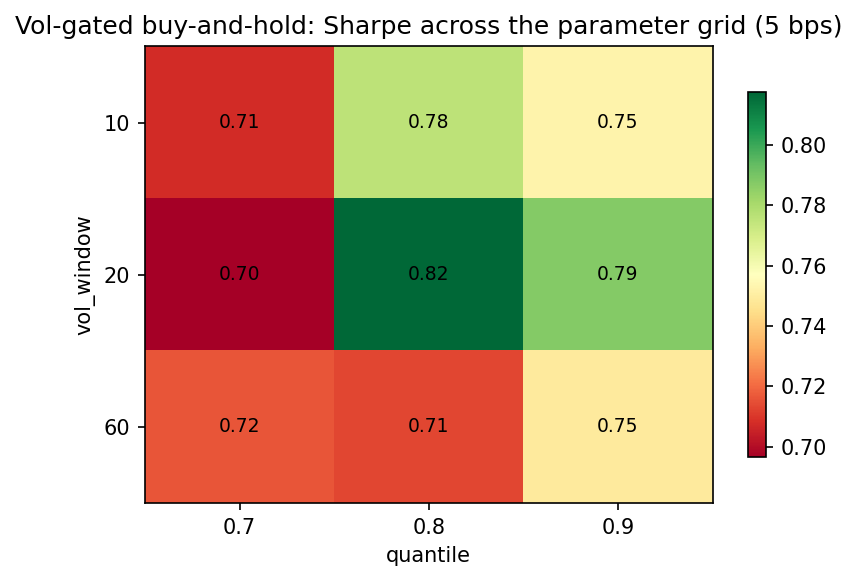
\includegraphics[width=0.6\textwidth]{spy_sensitivity.png}
\caption{Volatility-gate parameter grid (Sharpe of gated buy-and-hold, 5
bps). A plateau, not a peak: every cell beats buy-and-hold's 0.55, so the
headline configuration (20d, $q{=}0.8$) is not a tuned artifact.}
\label{fig:sens}
\end{figure}

Two nuisance checks complete the picture. Across bootstrap block lengths
$\{5, 21, 63\}$, $P(\le 0)$ for the headline comparisons moves by less than
$0.03$ (e.g.\ volatility gate vs.\ buy-and-hold: $0.18 / 0.19 / 0.18$).
Across walk-forward schedules ($\{$expanding, rolling$\} \times \{126,
252\}$-day refits), the volatility gate's Sharpe stays within $0.70$--$0.78$.
No conclusion hinges on either constant.

\section{Results: multi-asset (SPY/TLT/GLD)}

Each asset is gated by its own independently fitted regime model; the
baseline is the equal-weight portfolio. Table~\ref{tab:ma} and
Figures~\ref{fig:mawealth}--\ref{fig:mafrontier} report the results.

\begin{table}[H]
\centering
\caption{Multi-asset universe (equal-weight SPY/TLT/GLD), out-of-sample
2010--2026, net of 5 bps, cash leg active.}
\label{tab:ma}
\small
\begin{tabular}{lrrrrr}
\toprule
Strategy & Ann.\ ret. & Ann.\ vol. & Sharpe & Max DD & Turnover \\
\midrule
vol20q80\_bh    & 7.5\% & 7.5\% & 0.82 & $-12.7\%$ & 5.0$\times$ \\
buy\_and\_hold  & 8.9\% & 9.3\% & 0.81 & $-22.7\%$ & 0.06$\times$ \\
hmm2p\_b10\_bh  & 6.1\% & 5.9\% & 0.79 & $-10.2\%$ & 4.9$\times$ \\
hmm2p\_b05\_bh  & 6.2\% & 6.5\% & 0.74 & $-12.1\%$ & 7.4$\times$ \\
hmm2p\_bh       & 6.3\% & 6.8\% & 0.72 & $-12.2\%$ & 11.3$\times$ \\
vol20q80\_trend & 5.7\% & 6.1\% & 0.72 & $-13.3\%$ & 9.2$\times$ \\
hmm2p\_b20\_bh  & 5.0\% & 5.1\% & 0.71 & $-8.3\%$  & 2.4$\times$ \\
hmm2\_bh        & 6.0\% & 7.3\% & 0.64 & $-15.0\%$ & 9.5$\times$ \\
trend\_200d     & 5.8\% & 7.2\% & 0.63 & $-12.6\%$ & 8.4$\times$ \\
\bottomrule
\end{tabular}
\end{table}

\begin{figure}[H]
\centering
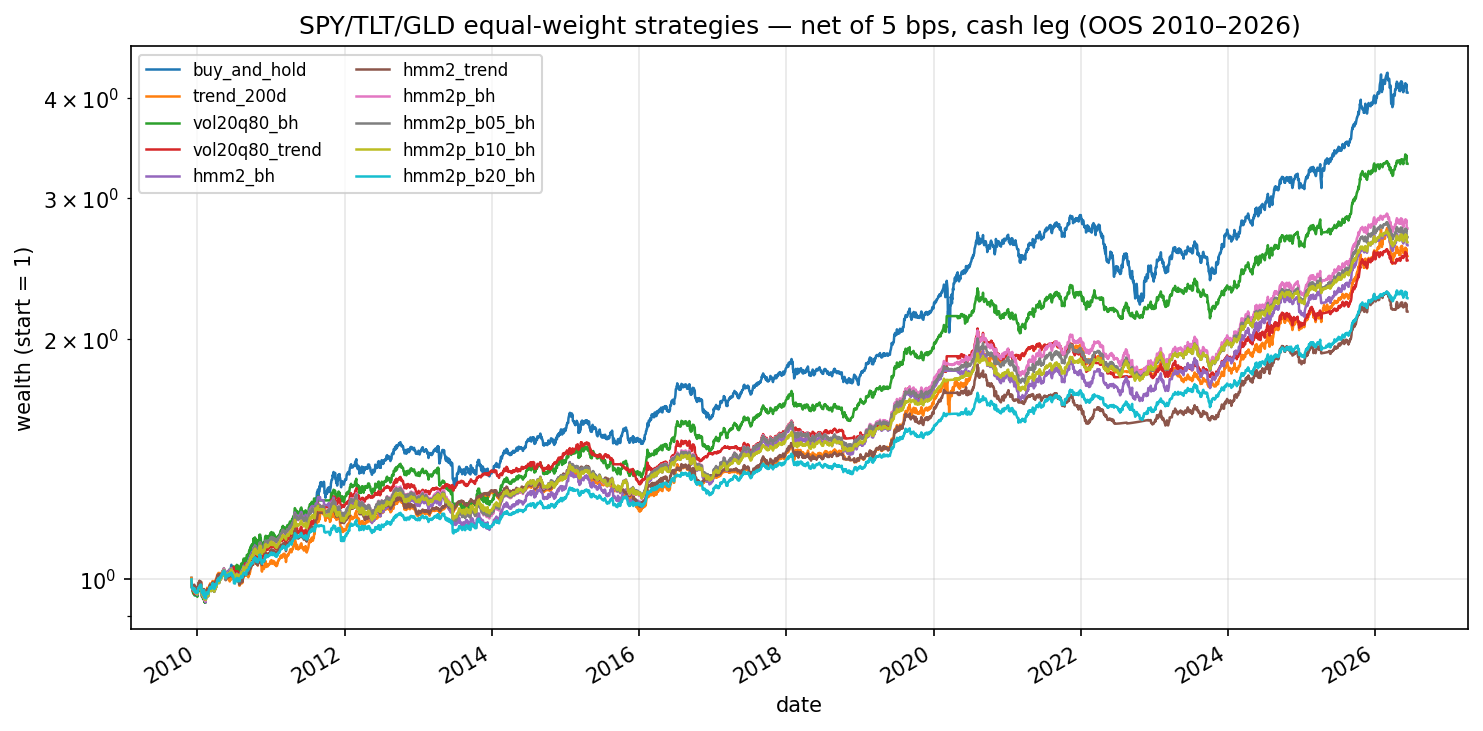
\includegraphics[width=\textwidth]{multiasset_wealth.png}
\caption{Multi-asset cumulative wealth, net of 5 bps with the cash leg. The
equal-weight portfolio is already smooth; gated variants trade return for
further drawdown reduction.}
\label{fig:mawealth}
\end{figure}

The headline result is negative and informative: the diversified equal-weight
portfolio achieves excess Sharpe 0.81 with a $-22.7\%$ maximum drawdown, and
no gated variant improves on it with any confidence (volatility gate:
$\Delta$Sharpe $+0.01$, $P(\le 0) = 0.46$; hard HMM gate: $-0.16$,
$P(\le 0) = 0.87$). The strongest bootstrap signals in the study are
orderings \emph{within} the gated family: the volatility heuristic beats the
hard HMM gate ($+0.17$, $P(\le 0) = 0.04$), and soft scaling beats hard
gating ($P(\text{hard} \ge \text{soft}) = 0.045$).

\begin{figure}[H]
\centering
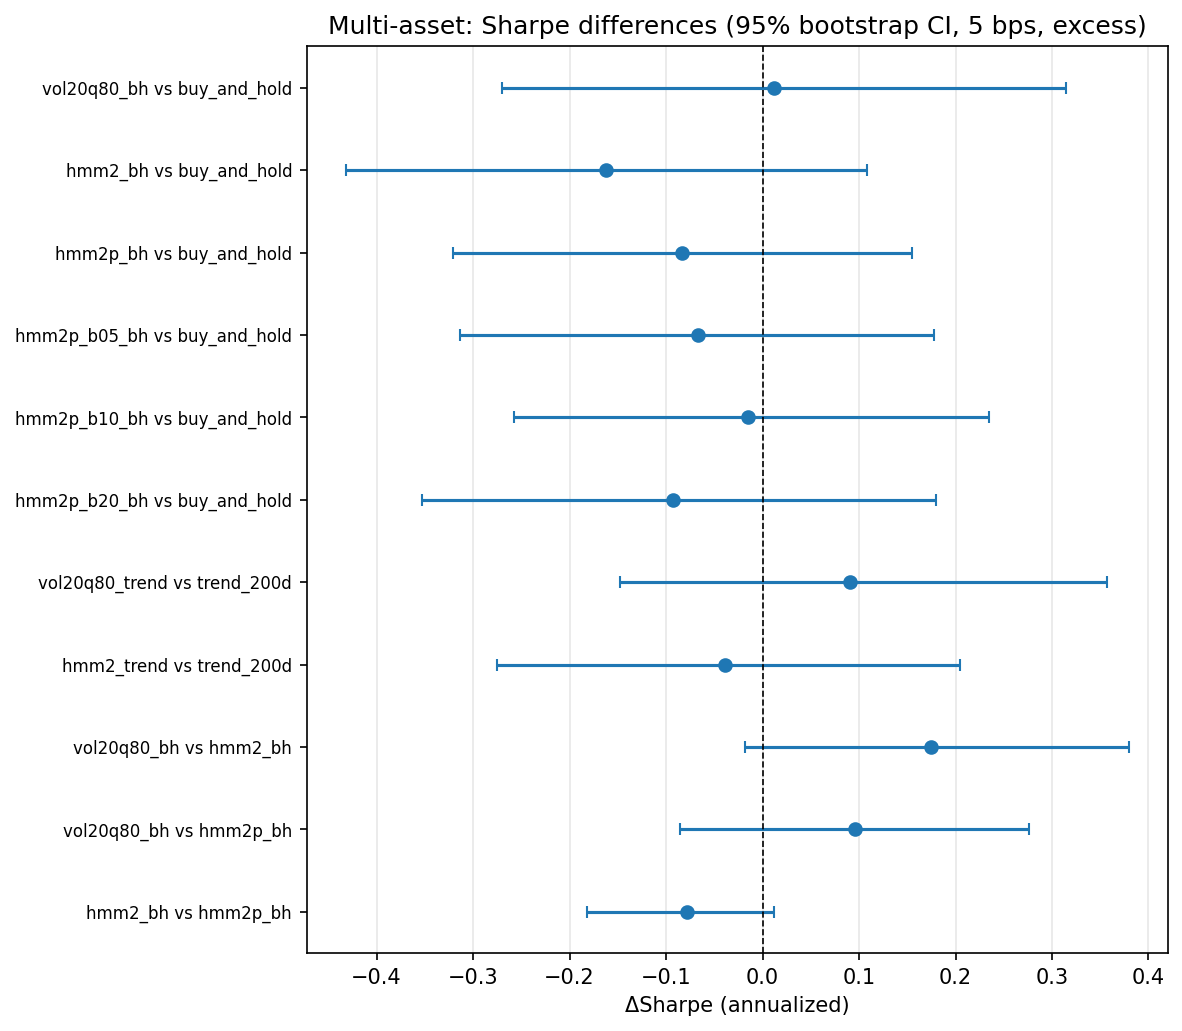
\includegraphics[width=0.85\textwidth]{multiasset_bootstrap.png}
\caption{Multi-asset Sharpe differences with 95\% paired-bootstrap intervals.
Nothing beats diversified buy-and-hold; the informative orderings are within
the gated family (heuristic $>$ hard HMM; soft $>$ hard).}
\label{fig:maboot}
\end{figure}

\begin{figure}[H]
\centering
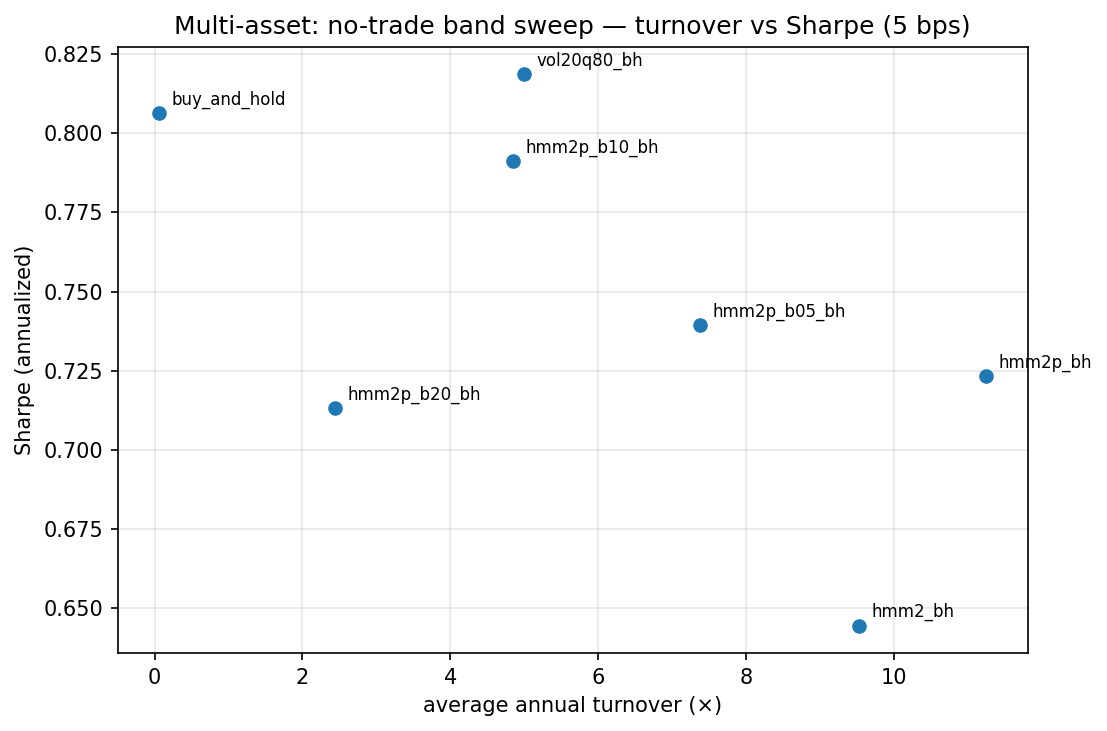
\includegraphics[width=0.8\textwidth]{multiasset_frontier.png}
\caption{Multi-asset turnover--Sharpe frontier. The band sweep moves the HMM
family from clearly worse than buy-and-hold (hard gate: Sharpe 0.64 at
$9.5\times$/yr) to nearly matching it: $\delta{=}0.10$ gives Sharpe 0.79 with
half the drawdown ($-10\%$ vs.\ $-23\%$) on $4.9\times$/yr turnover;
$\delta{=}0.20$ cuts the drawdown to $-8\%$ on $2.4\times$/yr.}
\label{fig:mafrontier}
\end{figure}

\section{Discussion and conclusions}

\begin{enumerate}
  \item \textbf{Regime gating is crash insurance.} In every configuration
        tested it cuts deep drawdowns at some cost in return, and the
        drawdown improvement --- unlike the Sharpe improvement --- appears in
        every sub-period. Sharpe gains of $\approx 0.15$ never clear paired
        bootstrap scrutiny on 21 years of daily data; claims of regime-based
        Sharpe enhancement at this sample size deserve suspicion.
  \item \textbf{Complexity did not pay.} The HMM never beat the volatility
        heuristic where both worked (SPY: $\Delta$Sharpe $+0.01$) and was
        clearly worse in the multi-asset setting ($P(\le 0) = 0.04$ for the
        heuristic--HMM comparison), where it trades bond and gold volatility
        states that are not reliably associated with negative returns the way
        equity volatility is.
  \item \textbf{Diversification first.} The cheapest ``regime model'' in the
        study is holding three lowly-correlated assets: equal-weight
        SPY/TLT/GLD matches the best gated single-asset Sharpe at near-zero
        turnover. This is established here with a proper cash leg, so it is
        not an artifact of uncompensated cash.
  \item \textbf{If using a probabilistic model: scale, band, do not
        threshold.} The ordering hard gate $<$ soft scaling $<$ banded
        scaling holds in both universes. Banding fixes the cost fragility
        that made the HMM strictly worse at 20 bps, and multi-asset it
        converts the HMM from a detractor into cheap insurance.
  \item \textbf{The findings are not nuisance-parameter artifacts} ---
        stable across bootstrap block lengths and walk-forward schemes and
        cadences.
\end{enumerate}

\section{Limitations}

The cash conversion uses the discount-yield approximation $y/100/252$;
negligible at historical yields, but documented rather than eliminated. The
band levels were swept, not optimized, yet the sweep grid itself was chosen by
the authors; a pre-registered grid would be cleaner. Multi-asset gating is
per-asset and ignores cross-asset information. The data source is Yahoo
Finance, and the multi-asset sample covers roughly one and a half market
cycles. Finally, with about a dozen strategy variants, multiple-comparison
effects deserve formal treatment (e.g.\ deflated Sharpe ratios) once the
strategy set stops growing.

\section{Next steps}

\begin{enumerate}
  \item A \emph{joint multivariate} HMM on the SPY/TLT/GLD return vector,
        against the per-asset models used here --- testing whether
        cross-asset structure rescues the statistical approach.
  \item A deflated-Sharpe / multiple-comparison appendix.
  \item Block-bootstrap inference on drawdown-based metrics, the quantity
        regime gating actually improves.
\end{enumerate}

\appendix
\section{Reproducibility}

All results in this report regenerate from a clean checkout with:

\begin{verbatim}
pip install -e ".[models,data,notebooks,dev]"
pytest                                                  # 102 tests
python experiments/run_regime_comparison.py configs/comparison_spy.yaml
python experiments/run_robustness.py       configs/comparison_spy.yaml
python experiments/run_regime_comparison.py configs/multiasset.yaml
python experiments/run_robustness.py       configs/multiasset.yaml
PYTHONPATH=src jupyter nbconvert --to notebook --execute \
    --inplace notebooks/0*.ipynb
\end{verbatim}

Experiment outputs land in \code{experiments/outputs/}, one directory per
experiment; the figures used here are produced by the notebooks into
\code{reports/figures/}. The methodological decision log is
\code{reports/decisions.md}; this document is compiled with
\code{make -C reports} (Tectonic).

\end{document}
